\documentclass[a4paper,11pt]{article}

\usepackage[T1]{fontenc}

\usepackage[utf8]{inputenc}

\usepackage[italian]{babel}

\usepackage{graphicx}

\usepackage{indentfirst}

\usepackage{amsmath,amssymb}

\usepackage{enumitem} 

\newcommand{\virgolette}[1]{``#1''}

\usepackage[margin=1in]{geometry} %Smaller margins

\usepackage{lmodern} %Vector PDF

\usepackage{siunitx}

\usepackage{xcolor}

\usepackage{colortbl}

\usepackage{multirow}

\usepackage{rotating}

\usepackage{booktabs}

\usepackage{longtable}

\usepackage{graphicx}
\graphicspath{ {../../Immagini/} }

\usepackage{wrapfig}

\usepackage{siunitx} % Per unità di misura in generale e la corretta rappresentazione dei numeri.

\usepackage{gensymb} % Per il simbolo di gradi


\begin{document}
	
	\begin{titlepage}
		\centering
		{\scshape\LARGE Laboratorio di Ottica, Elettronica e \\ Fisica Moderna \par}
		\vspace{1cm}
		{\scshape\Large Relazione di Laboratorio 3\par}
		\vspace{1.5cm}
		{\huge\bfseries Interferometro di Michelson\par}
		\vspace{2cm}
		
		{\Large\itshape Nicolò Cavalleri, Giacomo Lini e Davide Passaro
			
			(LUN12)}
		
		\vspace{5cm}
		\vfill
		
		\begin{abstract}
			Di seguito vengono riportate la procedura sperimentale, e l'analisi dei dati raccolti relativi a un esperimento compiuto con un Interferometro di Michelson. In particolare tramite il calcolo delle frange di interferenza dell'immagine prodotta viene determinata la lunghezza d'onda della luce emessa da un laser monocromatico. Altre grandezze fisiche rilevanti che questo apparato consente di mettere in evidenza sono l'indice di rifrazione dell'aria, la lunghezza dei pacchetti d'onda emessi da luce non monocromatica, e la differenza di lunghezza d'onda tra sorgenti differenti, nello specifico l'analisi è relativa al doppietto di sodio. Per ognuna di queste grandezze vengono riportate procedure sperimentali e risultati comprensivi di errore.
		\end{abstract}
		
		
		\vfill
		{\large \today\par}
		
	\end{titlepage}
	
	\newpage
	
	\section{Introduzione}
	L'interferometro di Michelson è uno strumento che sfrutta alcune proprietà  delle radiazioni luminose per metterne in evidenza alcune caratteristiche. In particolare sfruttando una combinazione di specchi semi-riflettenti e altri completamente riflettenti, come descritto nella sezione \ref{strum} è possibile individuare la lunghezza d'onda di una particolare sorgente a partire dalla figura di interferenza che risulta.	
	
	\begin{wrapfigure}{r}{0.5\textwidth}
		\vspace{-1cm}
		\caption{Fotografia dell'apparato sperimentale}
		\vspace{0.2cm}
		\centering
		\label{apparato}
		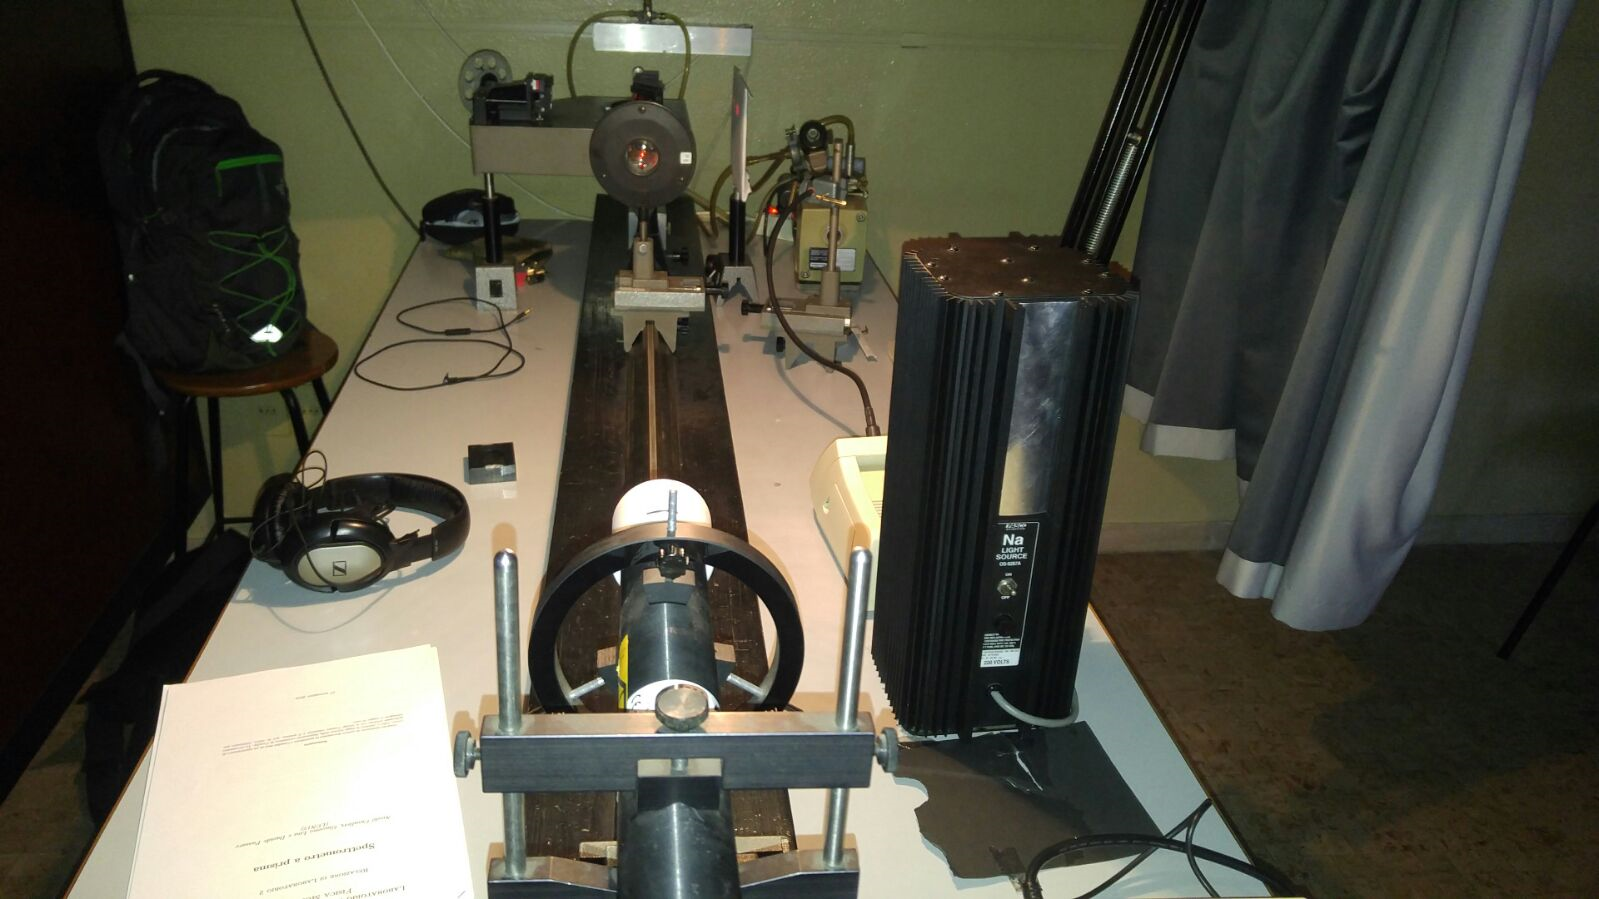
\includegraphics[width=0.48\textwidth]{apparato}
		\vspace{-0.5cm}
	\end{wrapfigure}
	
	La relazione che lega infatti la lunghezza d'onda $\lambda$ della sorgente, alla figura che si osserva muovendo uno dei due specchi riflettenti è la seguente:
	\begin{equation}\label{lambdana1}
		\lambda=\dfrac{2n_a\Delta x}{N_1}
	\end{equation}
	dove $n_a$ rappresenta l'indice di rifrazione dell'aria, $\Delta x$ indica lo spostamento di una delle due lenti e $N_1$ è il numero di massimi (o equivalentemente minimi) osservati mentre si spostava lo specchio di $\Delta x$.
	
	Quello che si osserva è che questa relazione consente di calcolare il valore di $\lambda$ a patto di conoscere il valore dell'indice di rifrazione $n_a$. Questo può a sua volta essere ricavato utilizzando una cameretta per il vuoto di lunghezza $d$ nota e contando le frange che si susseguono quando questa viene riportata alle condizioni dell'ambiente circostante. Vale infatti la relazione:
	\begin{equation}\label{indice_aria}
		2 (n_a - 1) d = N_2 \lambda
	\end{equation}
	dove $1$ è l'indice di rifrazione del vuoto, e $N_2$ è il numero di frange che si sono susseguite.
	
	Mettendo a sistema \ref{lambda} e \ref{indice_aria} si ricavano i valori sia di $\lambda$ che di $n_a$.
	
	Queste relazioni sono state ricavate dall'ipotesi che la luce emessa dalla sorgente nell'interferometro fosse monocromatica. Per luce non monocromatica, come una sorgente \virgolette{bianca} tramite un interferometro è possibile ricavare la lunghezza del pacchetto d'onda, ossia di una parte coerente con se stessa del treno d'onda. Attraverso questa strumentazione è possibile osservare in maniera diretta la lunghezza di un pacchetto di luce emessa.
	
	In modo simile è anche possibile risolvere due lunghezze d'onda molto vicine tra loro. Sfruttando relazioni descritte nella sezione \ref{proc}, siamo infatti stati in grado di determinare la differenza delle lunghezze d'onda dei due raggi più luminosi dello spettro del sodio.
	
	
%%%%%%%%%%%%%%%%%%%%%%%%%%%%%%%%%%%%%%%%%%%%%%%%%%%%%%%%%%%%%%%%%%%%%%%%%%%%%%%%%


	\section{Strumentazione} \label{strum}
\begin{figure}
	\caption{Schema interferometro}\label{interf}
	\centering
	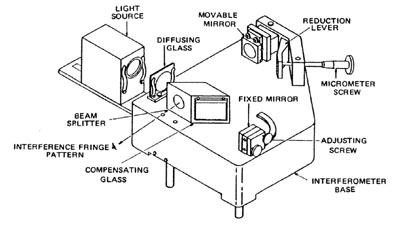
\includegraphics[width=0.95\textwidth]{interf}
\end{figure}
Poiché l'esperimento aveva più obiettivi la strumentazione ha coinvolto componenti diverse a seconda della misura che si stava effettuando. Ci sono stati però degli strumenti indispensabili per tutta l'esperienza. In generale però la strumentazione usata era composta da:
\begin{description}
	
	\item[Interferometro di Michelson] Questo è stato il principale e più importante strumento utilizzato. L'interferometro è stato utilizzato per creare figure di interferenza in modo controllato. La figura \ref{interf} rappresenta schematicamente un interferometro simile a quello usato nel laboratorio.\\
	È utile per la spiegazione delle componenti dell'interferometro descrivere il suo funzionamento. Dopo essere usciti dalla sorgente (\emph{light source}) i raggi di luce entravano un dispositivo a forma di prisma con i lati di vetro che aveva il compito di dividere in due il fascio di luce (\emph{beam splitter}).
	Questo era fisso alla base dell'interferometro (\emph{interferometer base}) ed era trasparente sui lati, per permettere il passaggio della luce. Al suo interno era presente uno specchio semi riflettente (con la parte riflettente posta verso l'interno), e tre vetri piani. Lo specchio semi riflettente e il vetro opposto ad esso erano angolati di $ 45\degree $ rispetto agli altri due. Mentre i due vetri opposti l'uno all'altro non avevano una funzione vera e propria, il vetro opposto allo specchio semi riflettente (\emph{compensating glass}) serviva per ovviare le differenze dei percorsi dei due raggi spezzati.\\
	Dopo essere stati divisi dal dispositivo sopra i raggi di luce procedevano per due strade diverse. Uno procedeva in avanti, verso uno specchio fisso (\emph{fixed mirror}). Questo era regolato in fase di calibrazione e lasciato fermo. Per la calibrazione erano presenti due viti (\emph{adjusting scew}) una che regolava la sua angolazione rispetto alla base dell'interferometro ed una che regolava la sua angolazione rispetto allo specchio mobile. Quindi, dopo essere stato riflesso dallo specchio fisso il vetro tornava indietro verso il \emph{beam splitter}. Il secondo raggio di luce invece procedeva verso lo specchio mobile (\emph{movable mirror}). La sua angolazione rispetto alla base dell'interferometro non era regolabile, quindi si può supporre che sia perfettamente perpendicolare. La posizione dello specchio mobile era regolabile attraverso una vite micrometrica (\emph{micrometer screw}). La precisione di questa era ulteriormente aumentata di un fattore cinque da un sistema di leve (\emph{reduction lever}). Quindi dopo essere riflesso dallo specchio mobile il raggio ritornava verso il \emph{beam splitter}.\\
	Una volta riincontrati i raggi erano quindi riflessi verso lo schermo (non rappresentato in figura) dove formavano una figura di interferenza.

\end{description}

\begin{description}
	
	\item[Laser] Era presente uno strumento che generava un raggio laser. Il funzionamento di questo strumento va oltre gli scopi dell'esperienza. Sul dispositivo erano presenti delle informazioni scritte dal costruttore, secondo cui il raggio generato sarebbe stato di $ 633\si{\nano\meter} $.
	\item[Lente] Per rendere il fascio di luce laser più visibile è stata usata una lente convergente con distanza focale molto piccola. La lente permetteva di allargare il fascio luminoso per distinguere meglio le frange di interferenza.
	\item[Cameretta per il vuoto] Per la misura dell'indice di rifrazione dell'aria è stato usata una cameretta per il vuoto. Questa è stata fissata tra il \emph{beam splitter} e lo specchio fisso e aveva due lati trasparenti per permettere il passaggio della luce. La camera interna (lunga $ \SI{5}{\centi\meter}$) era collegata tramite un sistema di valvole e tubi ad una pompa per il vuoto che permetteva di creare il vuoto e lentamente far rientrare l'aria.
	\item[Una lampada al sodio] Usata per misurare la differenza di lunghezza d'onda tra le due lunghezze più visibili.
	\item[Una sorgente di luce bianca] Usata per misurare le dimensioni dei pacchetti d'onda.
	\item[Schermo] Le figure di interferenza erano proiettate su uno schermo bianco. Erano a disposizione due schermi, uno retto da un piccolo piedistallo sul tavolo di lavoro e uno appeso al muro di fronte (a circa $ \SI{3}{\meter} $).
\end{description}

\section{Iter sperimentale}\label{proc}
L'iter sperimentale può essere diviso nelle singole procedure utilizzate per compiere le diverse misure che erano l'obbiettivo dell'esperienza.

\subsection{Lunghezza d'onda del laser}
La prima parte dell'esperienza richiedeva una misura della lunghezza d'onda del laser. Questa operazione era sensata poiché il laser è un fascio di luce monocromatico e quindi dotato di una sola lunghezza d'onda.

\subsubsection{Calibrazione dello specchio fisso}\label{calib}
Per la misura della lunghezza d'onda del raggio laser è stata necessaria una calibrazione dell'interferometro volta al rendere lo specchio fisso perfettamente perpendicolare allo specchio mobile. Questo è stato fatto in due fasi. Per avere una condizione di perpendicolarità entro qualche primo è stata tolta la lente convergente. Sullo schermo si vedevano dei punti luminosi\footnote{Questi erano causati non interferenza ma da riflessioni \emph{parassite} dovute a riflessioni non volute degli innumerevoli specchi e lenti presenti nell'apparato.} ma i due corrispondenti alle riflessioni principali erano chiaramente distinguibili. Attraverso le viti dello specchio fisso si è quindi corretta la posizione dello specchio fino a quando i due punti luminosi non erano sovrapposti. Si è quindi proceduto inserendo tra la sorgente luminosa e il \emph{beam splitter}  la lente convergente. Sullo schermo erano quindi visibili i punti più luminosi sovrapposti e ingranditi. Attraverso un ulteriore aggiustamento dello specchio fisso si è potuti arrivare ad una condizione di quasi perfetta perpendicolarità, arrivando a vedere le frange di interferenza.

\subsubsection{Misura}
La misura della lunghezza d'onda ha sfruttato la possibilità di poter variare la posizione dello specchio mobile e quindi la differenza di cammino ottico dei raggi di luce. In questo modo era possibile controllare l'interferenza dei raggi luminosi e farli interferire in modo costruttivo o distruttivo. In particolare, affinché una frangia scura sullo schermo (corrispondente all'interferenza distruttiva) sostituisca una luminosa (interferenza costruttiva) è necessario spostare lo specchio di 
\begin{equation}\label{delta}
	\Delta x = \dfrac{\lambda}{4n_a}
\end{equation}
dove $ \lambda $ è la lunghezza d'onda e $ n_a $ è l'indice di rifrazione dell'aria. Inoltre affinché una frangia chiara sostituisca una scura è necessario un ulteriore spostamento $ \Delta x $, da cui, per far si che una frangia chiara venga sostituita dalla successiva era necessario uno spostamento di $ 2\Delta x $.

Poiché però la lunghezza d'onda era poco più grande della sensibilità dello strumento (la sensibilità era di $ \SI{0.2}{\micro\meter} $ mentre la lunghezza d'onda era dell'ordine di grandezza di $ \SI{100}{\nano\meter} $) per ottenere una misura con un errore accettabile era necessario far scorrere molte (circa $ \num{200} $) frange e dividere lo spostamento finale per il numero di frange viste. In questo modo rigirando la formula \ref{delta} si ottiene la formula \ref{lambdana1} ossia:
\begin{equation}\label{lambdana}
	\lambda=\dfrac{2n_a\Delta x}{N_1}		
\end{equation}
dove $ N_1 $ è il numero di frange contate e le altre osservabili sono come prima.

\subsection{Indice di rifrazione dell'aria}
Per la misura dell'indice di rifrazione dell'aria è stata usata la cameretta per il vuoto. Questa è stata posta in modo fisso tra la \emph{beam splitter} e lo specchio mobile ed è stata collegata ad una pompa per il vuoto. Il cambio dell'indice di rifrazione ha causato una differenza di cammino ottico. Una volta praticato il vuoto, attraverso una valvola a spillo si è lentamente fatto rientrare l'aria e contemporaneamente si è contato il numero di frange di luce che si alternavano. Al termine del rientro dell'aria il cammino ottico del fascio di luce passante per la cameretta del vuoto è variato della quantità:
\begin{equation}\label{deltavuoto}
	\Delta s = 2(n_a-1)d
\end{equation}
dove $ d $ è la lunghezza della cameretta e $ n_a $ è l'indice di rifrazione dell'aria. Con un susseguirsi di $ N_2 $ fasci luminosi si ritrova quindi l'equazione \ref{indice_aria} che combinata con la \ref{lambdana} restituisce:
\begin{equation}\label{lambda}
	\lambda=\dfrac{2d\Delta x}{N_1 d + N_2 \Delta x}
\end{equation}
\begin{equation}\label{na}
	n_a=\dfrac{N_1 d}{N_1 d + N_2 \Delta x}
\end{equation}

\subsection{Lunghezza dei pacchetti d'onda}
Se la luce immessa nell'interferometro è non monocromatica, la luce emessa è costituita da pacchetti d'onda di lunghezza limitata non coerenti l'uno con l'altro. Posta quindi una sorgente di luce bianca, per misurare la lunghezza di uno di questi pacchetti era quindi necessario misurare lo spostamento tra una condizione di assenza di interferenza e l'altra. Questa misura si è rilevata essere la più difficoltosa in quanto le frange luminose erano difficilmente distinguibili e la condizione di interferenza era presente solo per un piccolissimo intervallo di differenza di cammino ottico.

Una volta trovato però si è potuto misurare la differenza di cammino ottico che in questo caso equivaleva esattamente alla lunghezza del pacchetto di luce. 

\subsection{Differenza di lunghezze d'onda}
Come si era potuto verificare nell'esperienza dello spettrometro a reticolo il sodio presenta due frange luminose molto vicine l'una all'altra ma chiaramente distinte. Con l'interferometro di Michelson è stato possibile misurare con più precisione la differenza di lughezza d'onda dei due fasci. In particolare, poiché le lunghezze d'onda sono molto vicine l'una all'altra, per certi valori di differenza di cammino ottico si osserva che le frange luminose di una delle lunghezze d'onda si sovrappongono perfettamente a quelle dell'altra. L'immagine è quindi quella di una netta figura d'interferenza. Variando la differenza di cammino ottico, è possibie però raggiungere anche una posizione in cui le frange chiare di una lunghezza d'onda coprono quelle scure dell'altra, creando sullo schermo una luce diffusa. In questa condizione si è variata la differenza di cammino ottico di
\begin{equation}\label{delta1}
	\Delta_1=2N_1\frac{\lambda_1}{2}=(2N_1+1)\frac{\lambda_2}{2}
\end{equation}
ovvero di un multiplo intero di una delle due lunghezze d'onda, e un numero dispari della metà della lunghezza d'onda dell'altro. Da questa relazione si ottiene quindi una equazione per ricavare $ N_1 $:
\begin{equation}\label{N1}
	N_1=\dfrac{\lambda_1}{2\left(\lambda_2-\lambda_2\right)}\;.
\end{equation}
Con lo stesso ragionamento si può trovare che la figura di interferenza ritorna ad essere visibile dopo una differenza di cammino ottico di:
\begin{equation}\label{delta2}
	\Delta_2=(2N_2+1)\frac{\lambda_1}{2}=2N_2\frac{\lambda_2}{2}
\end{equation}
e quindi 
\begin{equation}\label{N2}
	N_2=\dfrac{\lambda_1}{\left(\lambda_2-\lambda_2\right)}=2N_1 \, .
\end{equation}
Sostituendo la \ref{N1} nella \ref{delta1} e la \ref{N2} nella \ref{delta2} si ottiene quindi che:
\begin{equation}\label{deltas}
	\Delta_2=2\Delta_1=\dfrac{\lambda_2\lambda_1}{\lambda_2-\lambda_1}\approx\dfrac{\lambda^2}{\lambda_2-\lambda_1}
\end{equation}
dove $ \lambda $ è una stima di $ \lambda_1 $ o $ \lambda_2 $. Sperimentalmente però era molto più semplice distinguere le zone nella quale la diffusione era totale rispetto a quelle di interferenza. Quindi si è potuto facilmente misurare $ \Delta_2+\Delta_1=3\Delta_1 $ da cui si ottiene che:
\begin{equation}\label{delta-lambda}
	\left(\lambda_2-\lambda_1\right)=\dfrac{3\lambda^2}{6\Delta_1}
\end{equation}


\end{document}
